\section{\acrfull{soa} Design}

In the initial phase of WDIAS architecture, it proposed with a \acrfull{soa} as shown in the \cref{fi:proposed_soa_arch_design}. Mainly it consist of 4 modules, namely:
- Import modules
Import modules are using for integration of data from different source which come in different data formats.
- Export modules
Export modules are using for data dissemination with different format which may required for different type of operations.
- Extension modules
Extension modules are capable of providing the data assimilation functionalities by providing some of key functionalities such as transformation, interpolation and validation. While data assimilation, existing timeseries maybe modified or create new timeseries based on the system configurations.
- Adapter module
Adapter module is handling the complexity of integrating different data formats and storing them in the way that easy to search and retrieve.

\begin{figure}[htp]
    \centering
    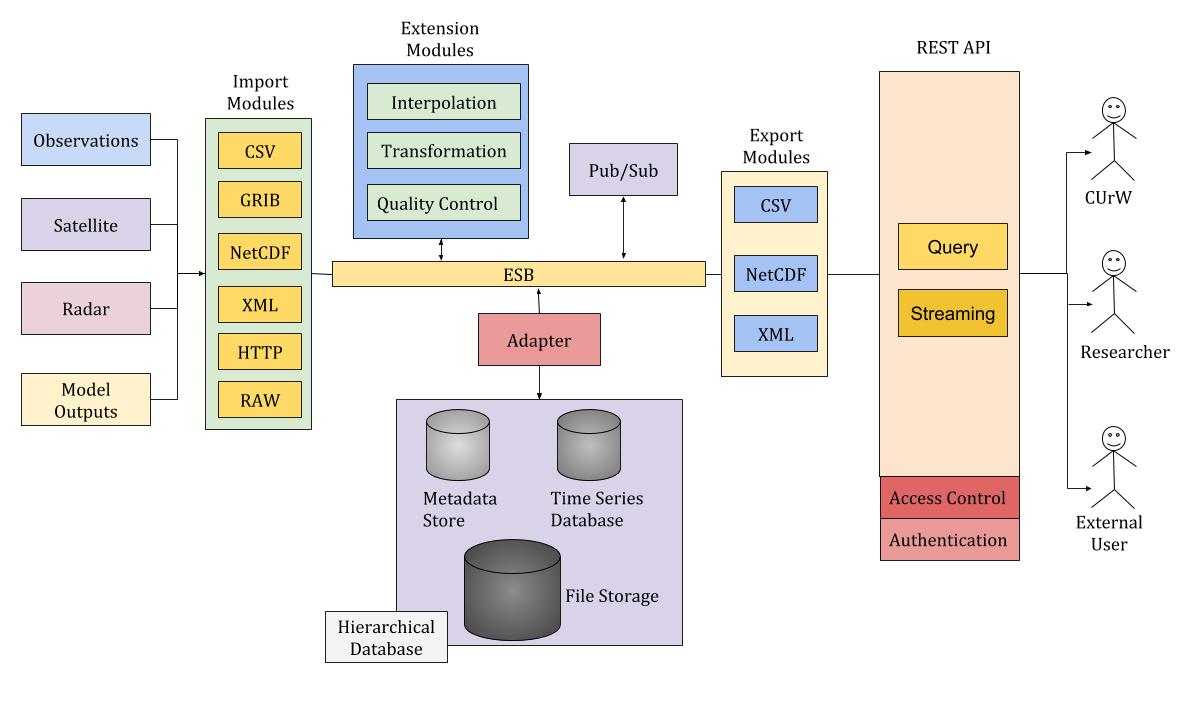
\includegraphics[width=1\textwidth]{method/soa/soa_v1.jpg}
    \caption{Service oriented architecture of \acrshort{wdias}.}
    \label{fi:proposed_soa_arch_design}
\end{figure}

In the second phase of \acrshort{wdias}, the proposed architecture changed to use with Actor model after consider into the disadvantage of using \acrshort{esb}.
